% !TEX root = DesignDocument.tex

\chapter{Sprint Results and Prototypes}    
    \hspace{7mm}This chapter will cover the contents of the tracked sprint progress, as well as any tables, figures, or listings
    pertaining to prototypes througout the development lifecycle.\\

    Sprints are being organized in two-week long segments, starting with sprint 0 being a planning and preparation phase.
    Each sprint detailed in this chapter will consist of:
    \begin{itemize} \item The Backlog \end{itemize}
    
        The backlog of a sprint is to be a list of the items that the development team wishes to accomplish in the duration
        of that sprint. Examples of backlog items could be ``Update documentation for (x)'' or ``Research best practices for (y)''.
        Trivial items, such as fixing a spelling mistake will not be listed on the sprint backlog.\\

    \begin{itemize} \item Successes \end{itemize}
        
        Items from the sprint backlog that were successfully accomplished.  Items listed under the ``Successes'' section
        may contain notes containing specific instructions as to how an issue was resolved.\\

    \begin{itemize} \item Failures \end{itemize}
        
        Items from the sprint backlog that were not successfully accomplished.  Items listed under the ``Failures'' section
        will be accompanied with a description detailing the manner of the failure.  Items to be considered as failed for the
        sprint are backlog items that were not addressed, backlog items that were not fully accomplished, backlog items that
        were attempted to be completed but found to be unreasonable or infeasible (in which case, the requirement needs revision),
        or additional problems that are introduced during the sprint cycle.\\
    \begin{itemize} \item Deliverables \end{itemize}
        
        A description of items from the sprint backlog, more specifically from the ``Successes'' section by the end of the
        sprint cycle, that are considered of value in the hands of the project client.  These are items that validate the 
        continuation of the development process.  Items that are considered to be ``Deliverable'' include, but are not 
        limited to, documentation, wireframes/designs, prototypes, demonstrations, and of course the final product.\\

    \begin{itemize} \item Sprint Review \end{itemize}
       
        An overviewing analysis of the results of the sprint.  This section is where items from the original backlog
        are evaluated and officially labeled as having either passed or failed it's acceptance criteria.\\

        Items having passed their acceptance criteria are appropriately labeled as ``Successes'' for the sprint and are 
        removed from the backlog moving forward to the next sprint development cycle.\\

        Items having failed their acceptance criteria are appropriately labeled as ``Failures'' for the sprint and are
        left on the backlog moving forward to the next sprint development cycle.  The reason for an item being labelled
        as failing for the sprint will be documented and  the item will be re-evaluated to ensure it remains feasible.\\  

    \begin{itemize} \item Sprint Retrospective \end{itemize}
        
        This section will contain both positive and negative remarks from the development team regarding topics such as 
        the rate at which work was completed and the ratio of successes to failures.  Reasons for failing items will be
        discussed and resolutions will be sought after.  If needed, failed items will be re-delegated to one or more 
        developers.\\

        This section also serves as an opportunity for the development team to evaluate the development process as a whole.
        Discussions can be held to suggest changes or improvements to how items are accomplished, or how the development
        process itself is managed.


    \newpage
    % !TEX root = ../../DesignDocument.tex

\section{Sprint 0 Report}
\label{sec:Sprint0_report}
    \subsection{Sprint Backlog}
    \label{sec:Sprint0_backlog}
        \begin{itemize}
            \item Define the toolchain
            \item Define the Minimum Viable Product (MVP)
            \item Create a data flow diagram to detail the MVP            
            \item Identify use cases and create user stories
            \item Estimate a timeline for the development process
        \end{itemize}

    \subsection{Successes}
    \label{sec:Sprint0_successes}
        \begin{itemize} \item Defined the MVP \end{itemize}
        \hspace{7mm}
        Upload a Maplesoft 3D object file to a website.  Have the website perform an automatic file conversion and 
        present the user with an AR Tag.  When the user views the AR Tag through an AR device, download and render 
        the 3D object file.

        \begin{itemize} \item Decided to develop with the Microsoft HoloLens being the primary supported AR device. \end{itemize}
        \hspace{7mm} 
        A conscious decision was made in accordance with current technologies and the Mobile Computing Grant awarded 
        to the South Dakota School of Mines and Technology that this service aims to satisfy to keep development 
        centered around the HoloLens and other Microsoft supported or compatible tools and services.

        \begin{itemize} \item Decided to use Azure for cloud hosting services \end {itemize}
        \hspace{7mm}The decision was between using Azure cloud services or Amazon Web Services. The development team voted to use Azure on the grounds that staying within the Microsoft development network would ensure compatibility with the primary target device, the Microsoft HoloLens, and ease development.

        \begin{itemize} 
            \item Created initial user stories 
            \begin{itemize}
                \item As a faculty member, I want:
                \begin{itemize} 
                    \item to upload a Maple file to a cloud server.
                    \item the Maple file to be automatically converted to an AR tag on the cloud server.
                    \item to be able to download the AR tag for my document from the cloud server.
                \end{itemize}
                \item As a user of this product, I want: 
                \begin{itemize}
                    \item to be able to view the AR tag through a Microsoft HoloLens to render a 3D model.
                \end{itemize}
            \end{itemize}
            \item Estimated tentative development timeline.
        \end{itemize}

    \subsection{Failures}
    \label{sec:Sprint0_failures}
        \begin{itemize} \item None \end{itemize}

    \subsection{Deliverables}
    \label{sec:Sprint0_deliverables}
        \begin{itemize} 
            \item Definition of the MVP
            \item Data flow diagram            
            \item User stories
            \item Defined toolchain
            \item A production timeline (tentative)
        \end{itemize}

    \subsection{Sprint Review}
    \label{sec:Sprint0_review}
        \hspace{7mm}
        All items on the sprint backlog were resolved in a timely, effective manner.

    \subsection{Sprint Retrospective}
    \label{sec:Sprint0_retrospective}
        \hspace{7mm}
        As this is the `setup' sprint, tasks and discussions were primarily limited to topics of planning and preparation.
        The team has been split into two subteams, a web team and a file conversion team.\\ 

        The web team was responsible for the development and management of the ASP.NET website.  This includes the
        structure and design of the website,  as well as the content, account security, organization, and data 
        storage/access.  Members are Daniel Hodgin, Savoy Schuler, and Brady Shimp.\\

        The file conversion team was responsible for research into file type and structure of commonly used 3D modeling
        software such as Maplesoft (TM), and file types that are render-able in commonly used Augmented Reality viewing devices.
        The expected result of the research is to devise a system to convert common 3D modeling software file types into either
        a common file type that is made render-able by commonly used Augmented Reality viewing devices, or a ubiquitous format
        that can then be exported to the necessary file format, depending on which Augmented Reality viewing device is 
        requesting the file. Members are Aaron Alphonsus, Cheldon Coughlen, and Kenneth Petry.
    \newpage
    % !TEX root = ../DesignDocument.tex

\section{Sprint 1 Report}
\label{sec:Sprint1_report}
    \subsection{Sprint Backlog}
    \label{sec:Sprint1_backlog}
    \begin{itemize}
        \item Design website wireframes 
        \item Implement a basic ASP.NET website to mirror wireframes
        \item Be able to upload simple files to the ASP.NET website's web root
        \item Research into widely used and compatible AR renderable file formats
    \end{itemize}

    \subsection{Successes}
    \label{sec:Sprint1_successes}
        \begin{itemize}
            \item Designed website wireframes
                \begin{itemize}
                    \item See figures x - y WARNING - FIX THIS %~\ref{fig:x} - ~\ref{fig:y}
                \end{itemize}
            \item Implemented a basic ASP.NET website to mirror wireframes
                \begin{itemize}
                    \item Hosted on a Microsoft Azure account belonging to Kenneth Petry
                \end{itemize}
            \item Research into widely used and compatible AR renderable file formats
                \begin{itemize}
                    \item Plan:
                        \begin{itemize}
                            \item When a user uploads a file, store it alongside a converted STL format
                            \item Upon access request, convert the STL file to the specified client type
                            \item The converted client type file will be stored with a limited lifetime
                            \item Serve the specified client type file to the user
                        \end{itemize}
                \end{itemize}
        \end{itemize}
    \subsection{Failures}
    \label{sec:Sprint1_failures}
        \begin{itemize} 
            \item Able to upload simple files to the ASP.NET website's web root
        \end{itemize}

    \subsection{Deliverables}
    \label{sec:Sprint1_deliverables}
    \begin{itemize}
        \item Data flow diagrams
            \begin{itemize} \item figures x - y WARNING - FIX THIS \end{itemize} %~\ref{fig:x} - ~\ref{fig:y}
        \item Website wireframe designs
            \begin{itemize} \item figures x - y WARNING - FIX THIS \end{itemize} %~\ref{fig:x} - ~\ref{fig:y}        
        \item A prototype of the website
    \end{itemize}

    \subsection{Sprint Review}
    \label{sec:Sprint1_review}
        \hspace{7mm}
        The only item listed as a failure for this sprint was the ability to upload a simple file
        to the web root folder of the ASP.NET website.  The code had been written by the end of the 
        development sprint cycle, but had yet commited to the repository and therefore was not 
        reviewed and approved.  Testing the functionality of the feature will be one of the primary 
        items in the next sprint development cycle.

    \subsection{Sprint Retrospective}
    \label{sec:Sprint1_retrospective}
        \hspace{7mm}
        The team is in agreement that the sprint went well.  The only item not fully completed was the simple
        file upload, which can be attributed to only one member of the web team working on it while the others
        create early project documents and are being introduced to developing in ASP.NET.  Items of interest 
        during the sprint include the arrival of the Occulus Rift VR headset.  This has sparked discussions of
        supporting hardware.  Future items to consider will be focused around the supplemental hardware needs 
        of the coming AR and VR devices such as:
        \begin{itemize}
            \item What are the minimum hardware specifications for a computer to operate the device?
            \item Where do we get a dedicated development computer with supported hardware?
            \item Where do we store the dedicated computer? 
        \end{itemize}

    \newpage
    % !TEX root = ../../DesignDocument.tex

\section{Sprint 2 Report}
\label{sec:Sprint2_report}
    \subsection{Sprint Backlog}
    \label{sec:Sprint2_backlog}
    \begin{itemize}
        \item Prepare for the first client presentation
        \item Working file conversion in a standalone application
        \item Test that simple file upload to the ASP.NET web root is operable
        \item Define the minimum specifications for a computer to operate pending AR and VR devices
        \item Talk to Professor Schrader about borrowing an old Opp Lab computer for development
        \item Talk to Dr. Rebenitsch about borrowing development work space 
    \end{itemize}

    \subsection{Successes}
    \label{sec:Sprint2_successes}
        \begin{itemize}
            \item Completed the first client presentation
            \item Able to convert file types in a standalone application
            \item Simple file upload to the ASP.NET web root folder is successful
            \item The minimum specifications for a development computer have been defined - ~\autoref{table:metatwosystemrequirements}
        \end{itemize}

    \subsection{Failures}
    \label{sec:Sprint2_failures}
        \begin{itemize}
            \item Unable to borrow development workspace from Dr. Rebenitsch
            \item Professor Schrader has old computers that do not meet the hardware requirements
            \item Professor Schrader is unable to provide us with a development computer that is 
            property of SD Mines without a reserved space  
            \item Textures associated with Maplesoft files are not kept after conversion
            \item The initial proposed software contract presented to SD Mines has been rejected
        \end{itemize}

    \subsection{Deliverables}
    \label{sec:Sprint2_deliverables}
    \begin{itemize}
        \item The first client presentation
        \item Demonstrate that standalone file conversion is operable
        \item Demonstrate that simple files are able to be uploaded to the ASP.NET web root
    \end{itemize}

    \subsection{Sprint Review}
    \label{sec:Sprint2_review}
        \hspace{7mm}
        The proposal to Dr. Rebenitsch to borrow development space in the SD Mines mobile computing lab has
        been rejected so attaining a private development space is still on the backlog moving forward.  Until
        then, Professor Schrader was unable to supply the team with a development computer, so long as the
        computer is property of SD Mines.\\

        Whether a development computer is or is not able to be issued, any of the old Opp Lab computers that Could
        be supplied by Professor Schrader do not meet the minimum hardware specifications for operating AR or VR
        devices.\\

        Through testing the standalone file conversion application, it was learned that Maplesoft files are unable
        to export texture or color properties upon conversion.\\

        The last and potentially largest roadblock encountered throughout this sprint development cycle is the 
        update that the initial software contract proposal that was presented to the Business Office of SD Mines
        has been rejected due to the language in the document specific to 
        \textit{InTouch L.L.C.} 
        retaining intillectual property for the project.  The contact at the SD Mines Business Office is adamant that 
        claims to intillectual property will not be negotiated.

    \subsection{Sprint Retrospective}
    \label{sec:Sprint2_retrospective}
        \hspace{7mm}
        The team is less than satisfied with the result of this sprint but optimistic looking forward.  The
        recorded failing items for this sprint are attributed to outside forces that are not related to the 
        development process.\\

        On the subject of finding a private development workspace, the unanimous decision of the development team is
        that until one is able to be reserved, working sessions involving the AR and VR equipment that is hardware
        dependent will have to be scheduled with a team member who owns a laptop that meets the minimum hardware
        specifications.\\

        On the subject of minimum hardware specifications, the unanimous decision of the development team is that a 
        portion of the project's hardware budget can be set aside for purchasing the necessary upgrades to a computer
        provided by Professor Schrader.  However, the issue of purchasing additional hardware is to be tabled until a
        private development space is able to be reserved.\\

        On the subject of the Maplesoft conversion, research is being done into how to make Maplesoft correctly export
        model color and texture information when the file is converted to an intermediary file type.\\ 

        On the subject of the software contract negotiations with SD Mines, the unanimous decision of the development 
        team is to abandon reliance on the funding from the SD Mines Mobile Computing Grant.  AR hardware will instead 
        be purchased via 
        \textit{InTouch L.L.C.}
        to continue development until completion.  Students shall be compensated as developers following a
        license purchase of the completed product by SD Mines.
    \newpage
    % !TEX root = ../DesignDocument.tex

\section{Sprint 3 Report}
\label{sec:Sprint3_report}
    \subsection{Sprint Backlog}
    \label{sec:Sprint3_backlog}
        \begin{itemize}
            \item Reserve a development workspace
            \item Familiarize with the Microsoft Hololens
            \item Software contract - avoid conflict of interest
            \item Get file conversion operable on the Azure cloud
            \item Research Azure blob storage and similar options for file storage
            \item Be able to download original and converted files the ASP.NET web root
        \end{itemize}

    \subsection{Successes}
    \label{sec:Sprint3_successes}
        \begin{itemize}
            \item Avoid conflict of interest
            \item Familiarize with Microsoft Hololens
            \item Research into Azure blob storage or similar options complete
            \item Able to minimally convert files from type A to type B once on the Azure cloud
            \item Able to download both the original and the converted files from the ASP.NET web root
        \end{itemize}

    \subsection{Failures}
    \label{sec:Sprint3_failures}
        \begin{itemize}
            \item Unable to reserve a development workspace
            \item File conversion on the Azure cloud is not an automatic process
        \end{itemize}

    \subsection{Deliverables}
    \label{sec:Sprint3_deliverables}
        \begin{itemize}
            \item Software contract
            \item Demonstrate that file conversion is operable on the cloud
            \item Demonstrate the basic ability to download documents from the web root folder
        \end{itemize}

    \subsection{Sprint Review}
    \label{sec:Sprint3_review}
        \hspace{7mm}
        A private development workspace is still yet to be reserved.\\

        Conflicts with the SD Mines Buissiness Office have been resolved.  A miscommunication resulted in their
        understanding that the development team intended to be temporarily employed by SD Mines for the duration
        of the 2017-18 academic year to receive funds.  Following policy would then require that all IP be retained
        by SD Mines and not \textit{InTouch L.L.C.}  A problem now arises in that Dr. McGough serves as the PI for
        the SD Mines Mobile Computing Grant and has a percent stake ownership in \textit{InTouch L.L.C.}  Forwarding
        any money from the Mobile Computing Grant to \textit{InTouch L.L.C.} presents itself as a conflict of interest.\\
        
        The Microsoft Hololens arrived and 3D files are able to be tested for AR compatibility.  Upon completing
        the gesture recognition tutorial, it was learned that the Hololens only supports one user account.  To
        change accounts is to factory reset the device and redo setup with a different user account.\\

        The question of file storage space was presented.  Microsoft ImagineX student development accounts do not
        offer space for document storage.  Research was done into the compatibility of Azure blob storage with 
        ImagineX student development accounts and similar options.\\
        
        Files that are uploaded to the ASP.NET web root folder are able to be successfully converted to an alternate
        file format.  Both the original file and the converted file are able to be downloaded from the ASP.NET web root
        folder.  The file conversion process must currently be invoked manually.\\

    \subsection{Sprint Retrospective}
    \label{sec:Sprint3_retrospective}
        \hspace{7mm}
        The team is mostly satisfied with the progress of the sprint.  The only failing items are automatic file
        conversion and reserving a private development workspace.\\

        On the subject of finding a private development workspace, the decision remains unanimous that until one 
        is able to be reserved, working sessions involving the AR and VR equipment that is hardware dependent 
        will have to be scheduled with a team member who owns a laptop that meets the minimum hardware
        specifications.\\

        On the subject of conflicts of interest, the unanimous decision between Dr. McGough and the representatives
        of \textit{InTouch L.L.C.} is that South Dakota Board of Regents policy will be followed to the letter.
        Including a reduced stake in company ownership and leaving decisions regarding purchase orders with the SD 
        Mines Mobile Computing Grant funds up to another SD Mines faculty member who is a signer for the grant.\\
        
        On the subject of Hololens accounts, the unanimous decision of the development team is that a Microsoft
        account will be created and used for the development of this project.  Once development is complete, the 
        device will be reset and returned to SD Mines for configuration.\\

        On the subject of file storage space, options considered were Microsoft OneDrive and Azure blob storage.
        Microsoft OneDrive only allows interfacing via the web from business subscriptions which remain too 
        expensive for the budget of this project and would add a large overhead cost to any future clients.
        Azure blob storage is offered (5 GB per month) for free for a year for a standard trial subscription.
        The unanimous decision of the development team is that when the point in the development process is reached
        where files need to be stored and maintained, the team's Azure subscription will be changed from the 
        ImagineX student developer subscription to the standard free subscription.\\
        
        On the subject of automatic file conversion, it is known that the process needs to be made synchronous
        in order to be automatically invoked when a file is uploaded to the ASP.NET web site.  The item will be
        presented in the backlog of the following sprint.

    \newpage
    % !TEX root = ../DesignDocument.tex

\section{Sprint 4 Report}
\label{sec:Sprint4_report}
    \subsection{Sprint Backlog}
    \label{sec:Sprint4_backlog}
        \begin{itemize}
            \item Generate unique QR codes on a for each uploaded file
            \item Refine development timeline in accordance with the feedback from the client presentation
        \end{itemize}

    \subsection{Successes}
    \label{sec:Sprint4_successes}
        \begin{itemize}
            \item Developed a plan for generating unique QR codes for each uploaded file
            \item Refined the development timeline to postpone multi-user features in lieu of a more basic MVP
        \end{itemize}

    \subsection{Failures}
    \label{sec:Sprint4_failures}
        \begin{itemize}
            \item Unique QR code generation is not yet implemented 
        \end{itemize}

    \subsection{Deliverables}
    \label{sec:Sprint4_deliverables}
    \begin{itemize}
        \item Demonstrate unique QR code generation on a per-file basis
        \item A revision of the development timeline
    \end{itemize}

    \subsection{Sprint Review}
    \label{sec:Sprint4_review}

    \subsection{Sprint Retrospective}
    \label{sec:Sprint4_retrospective}

    \newpage
    % !TEX root = ../../DesignDocument.tex

\section{Sprint 5 Report}
\label{sec:Sprint5_report}
    \subsection{Sprint Backlog}
    \label{sec:Sprint5_backlog}
        \begin{itemize}
            \item Reserve a development workspace
            \item Prepare and give the second client presentation            
            \item Research into Collada file type for Maple textures
            \item Continue work to implement automatic QR code generation
            \item Update project documentation in accordance to the Senior Design Fall 2017 requirements
        \end{itemize}

    \subsection{Successes}
    \label{sec:Sprint5_successes}
        \begin{itemize}
            \item Collada file type research
            \item The second client presentation
            \item Update project documentation for Senior Design
        \end{itemize}

    \subsection{Failures}
    \label{sec:Sprint5_failures}
        \begin{itemize}
            \item Unable to reserve a development workspace
            \item Continue to implement automatic QR code generation
        \end{itemize}

    \subsection{Deliverables}
    \label{sec:Sprint5_deliverables}
        \begin{itemize}
            \item The second client presentation
            \item Project documentation for the 2017 Fall semester
        \end{itemize}

    \subsection{Sprint Review}
    \label{sec:Sprint5_review}
        \hspace{7mm}
        A private development workspace is still yet to be reserved.\\

        Unique QR codes are able to be manually generated given a file path.  A plan exists for automating
        the process but is not yet implemented.\\
        
        Collada file type research shows that the Collada .dae file format should be our intermediary file type.

    \subsection{Sprint Retrospective}
    \label{sec:Sprint5_retrospective}
        \hspace{7mm}
        The development team is in agreement that this was a successful sprint.  The amount of
        content developed during this sprint was minimal in lieu of items such as the client 
        presentation and ensuring the completeness of the documentation required for the 2017
        Fall semester.\\
        
        On the subject of finding a private development workspace, the decision remains unanimous that until one 
        is able to be reserved, working sessions involving the AR and VR equipment that is hardware dependent 
        will have to be scheduled with a team member who owns a laptop that meets the minimum hardware
        specifications.\\

        On the subject of fully implementing QR code generation, the decision remains that 
        the feature is not crucial to the function of the MVP and can be postponed until after the delivery
        of the MVP to be implemented.\\

        On the subject of Collada .dae file type research, The upside of using COLLADA is that it doesn't just 
        contain `geometry data' but also information about motion, light sources, textures etc. COLLADA also 
        has a lot of applications that support it - meaning that being able to export to it and convert it to 
        other formats will probably be easy. The downside to using COLLADA will probably not be an issue. 
        COLLADA has a complex file structure which makes parsing and loading it a challenge. However, at least 
        at this point, it doesn't look like this project will need that. Also, there are a few libraries to 
        help out with this, if needed.\\


    \newpage
    \section{Prototypes}
    %! TEX root = ../../DesignDocument.tex

%% Add in images of prototypes
%% Add good reference labels to each prototype
%% Go back through sprint documentation and reference prototype labels

%% In reality it shouldn't take that long but I'm pretty tired and just don't want to do it right now
    \newpage
    \section{Final Designs}
    %! TEX root = ../../DesignDocument.tex
\hspace{7mm}
The following images show the final Phase One version of the project. 
\subsection{Public Content}
    \hspace{7mm} The Public Content homepage displays all publicly viewable content with options for searching and filtering the table. Clicking on a row will expand the row to reveal options. 
    \label{fig:final_public_content_page}
    \begin{figure}[H]
        \centering 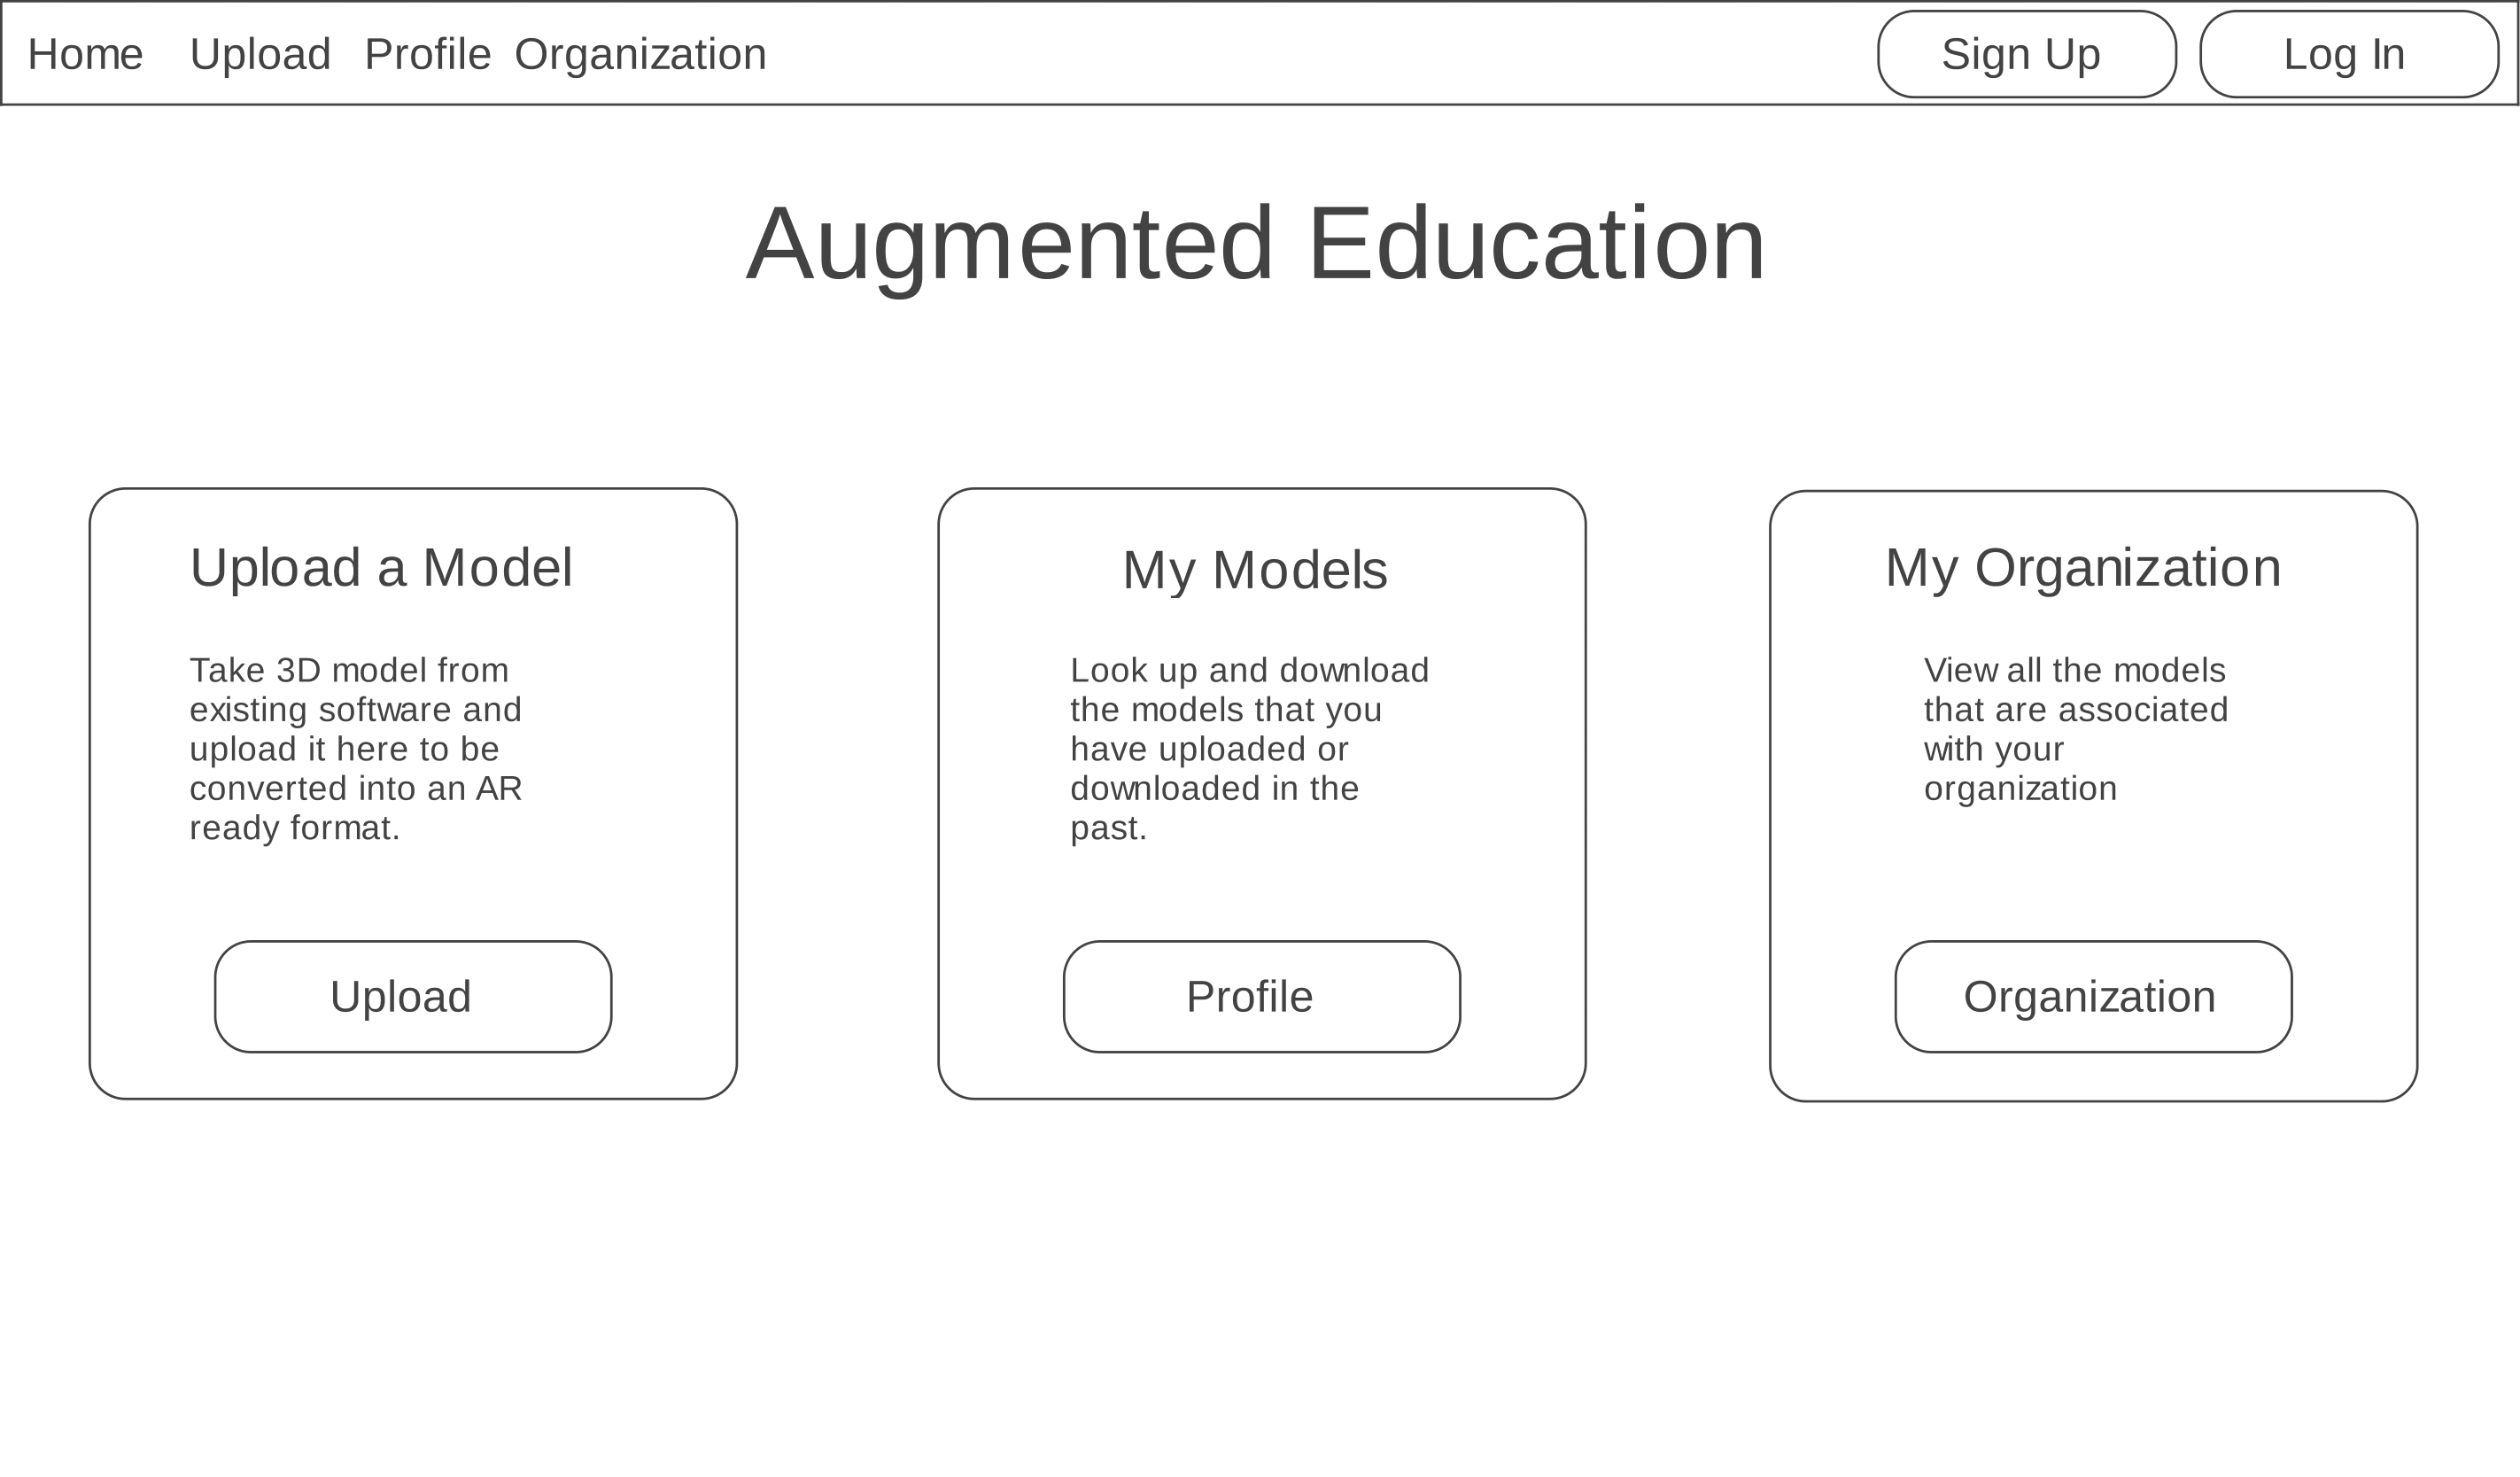
\includegraphics[width=0.6\linewidth]{Home}
        \caption{Final design for the Public Content homepage}
    \end{figure}

\subsection{Upload Page}
    \hspace{7mm} The page where a user can fill out a form 
    that allows them to browse to a 3D model file on their computer and upload
    it to the ASP.NET website under their user account.
    \ \\
    \label{fig:final_upload_page}
    \begin{figure}[H]
        \centering 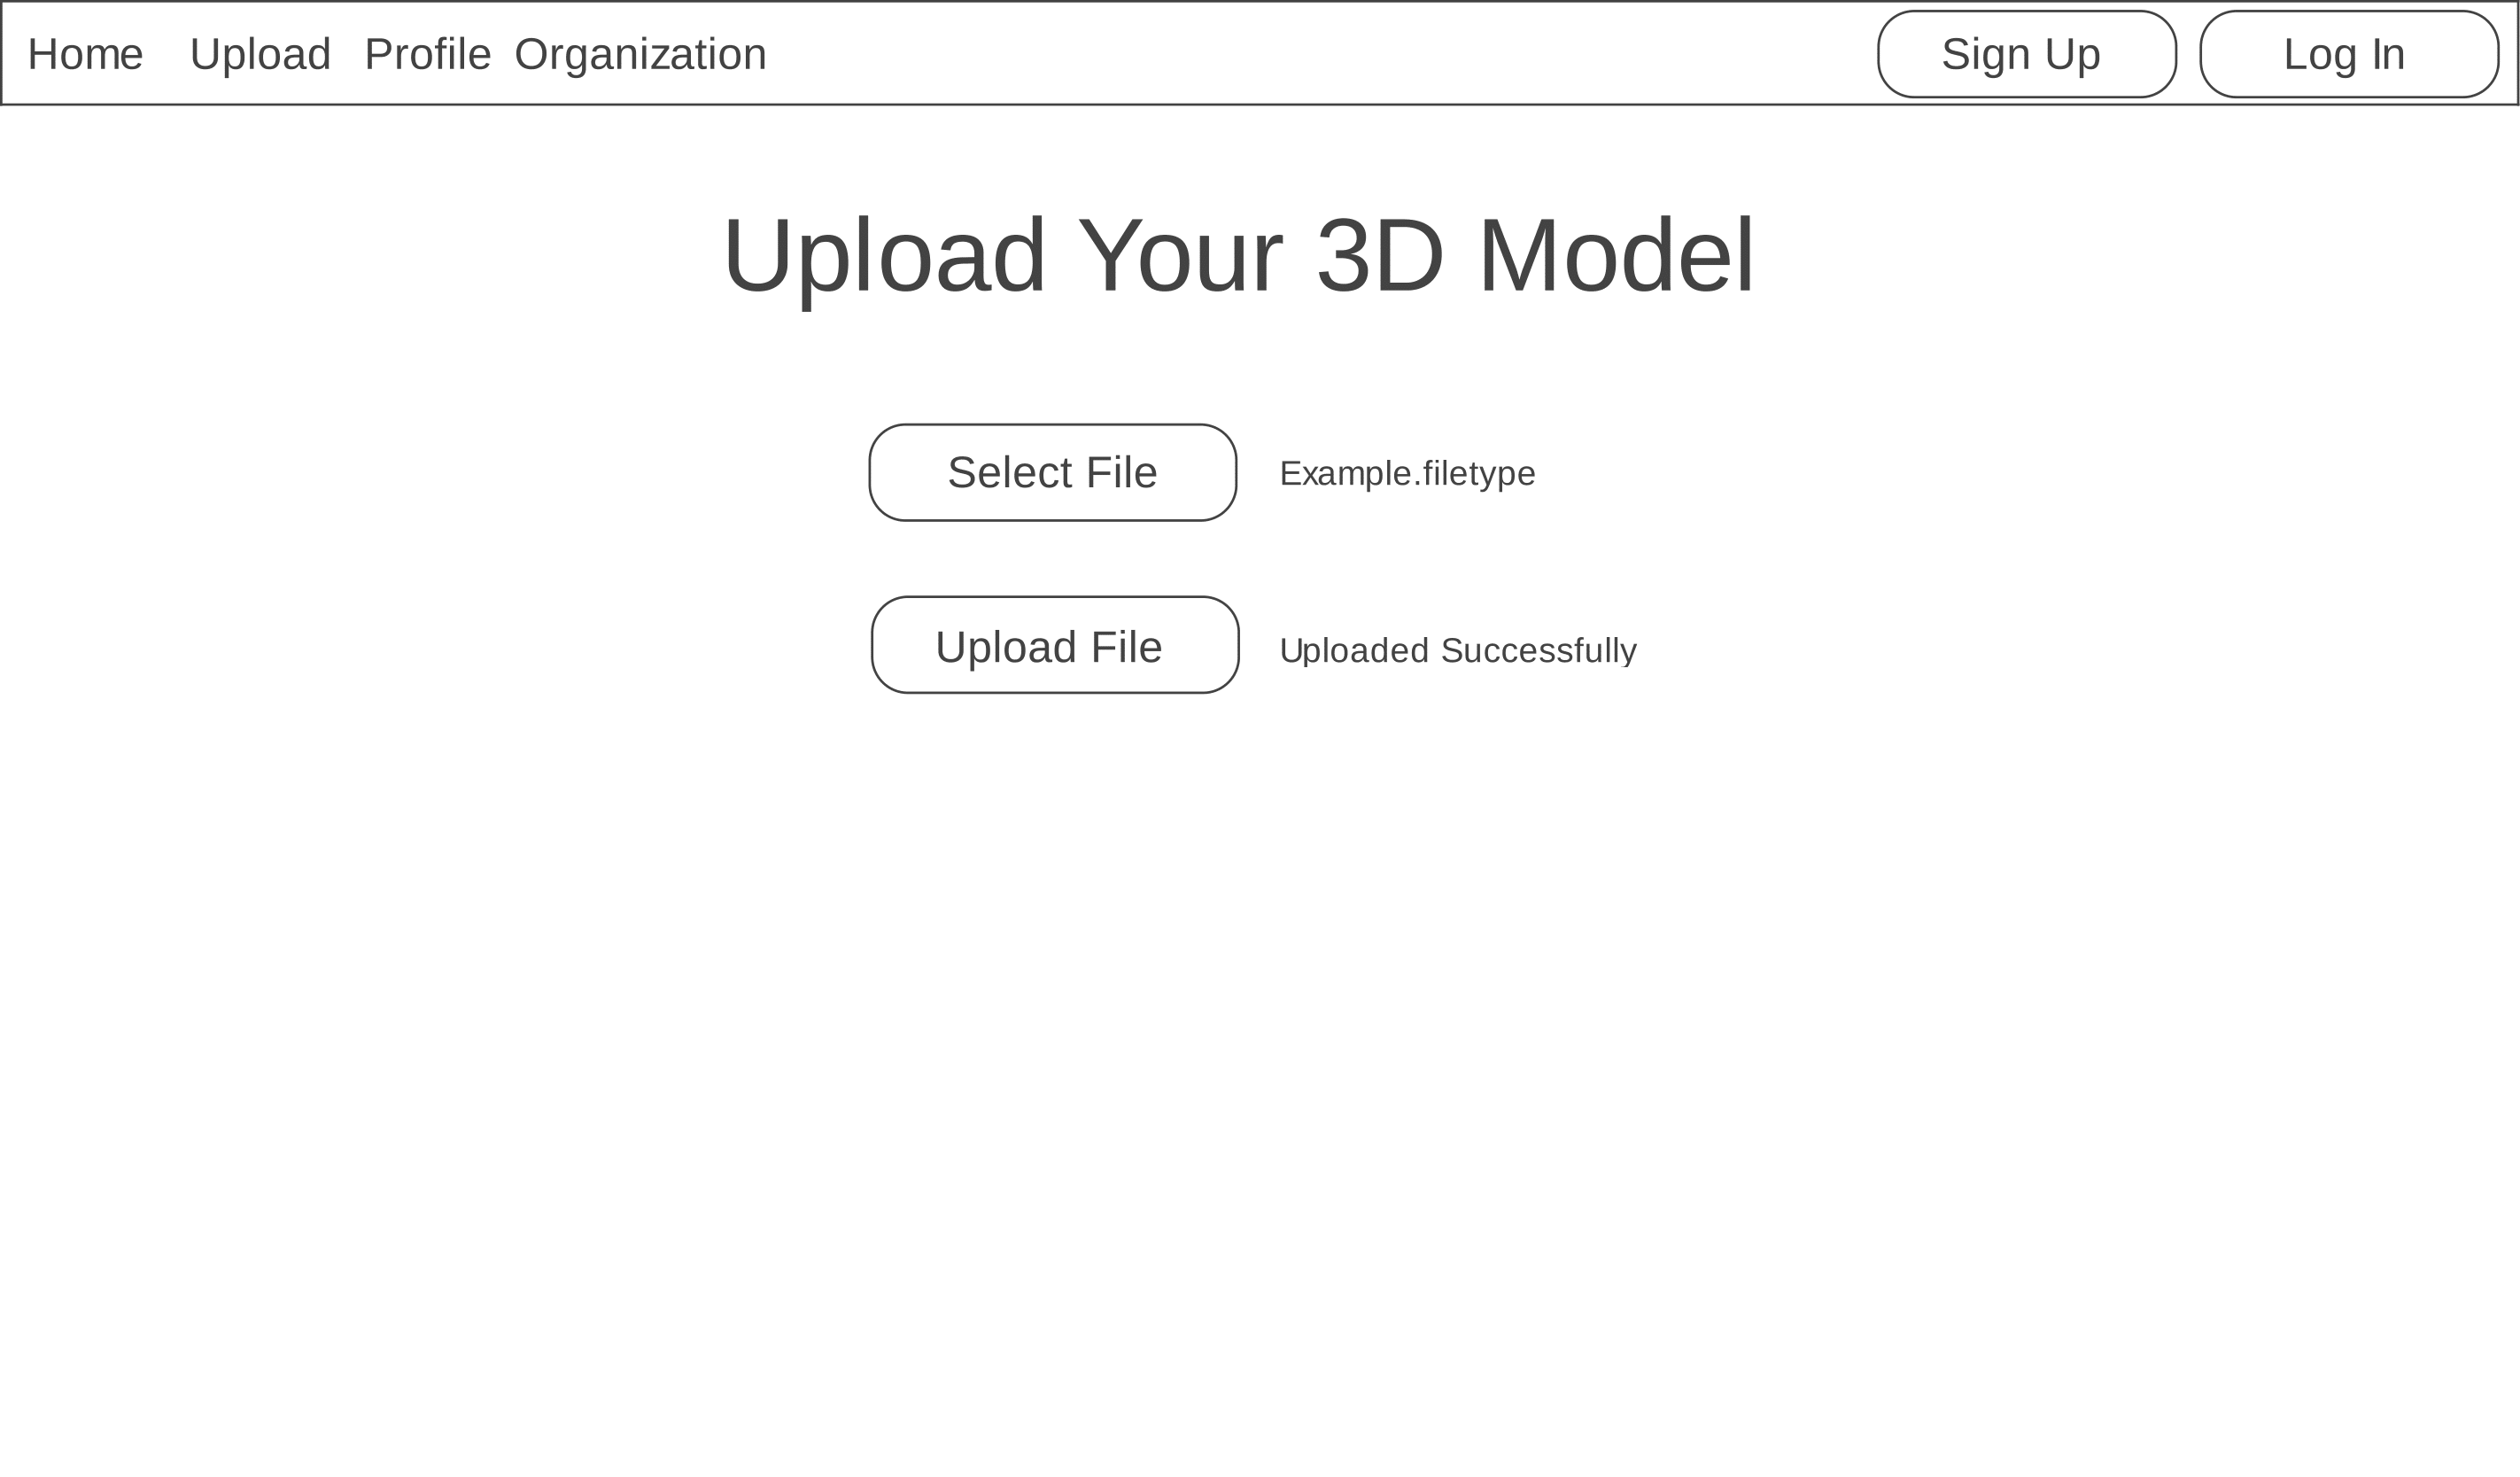
\includegraphics[width=0.6\linewidth]{Upload}
        \caption{Final design for the Upload page}
    \end{figure}

\subsection{My Content}
    \hspace{7mm}
    A page where a user may view all of their public and private files being stored 
    on the cloud.
    \ \\
    \label{fig:final_my_content_page}
    \begin{figure}[H]
        \centering 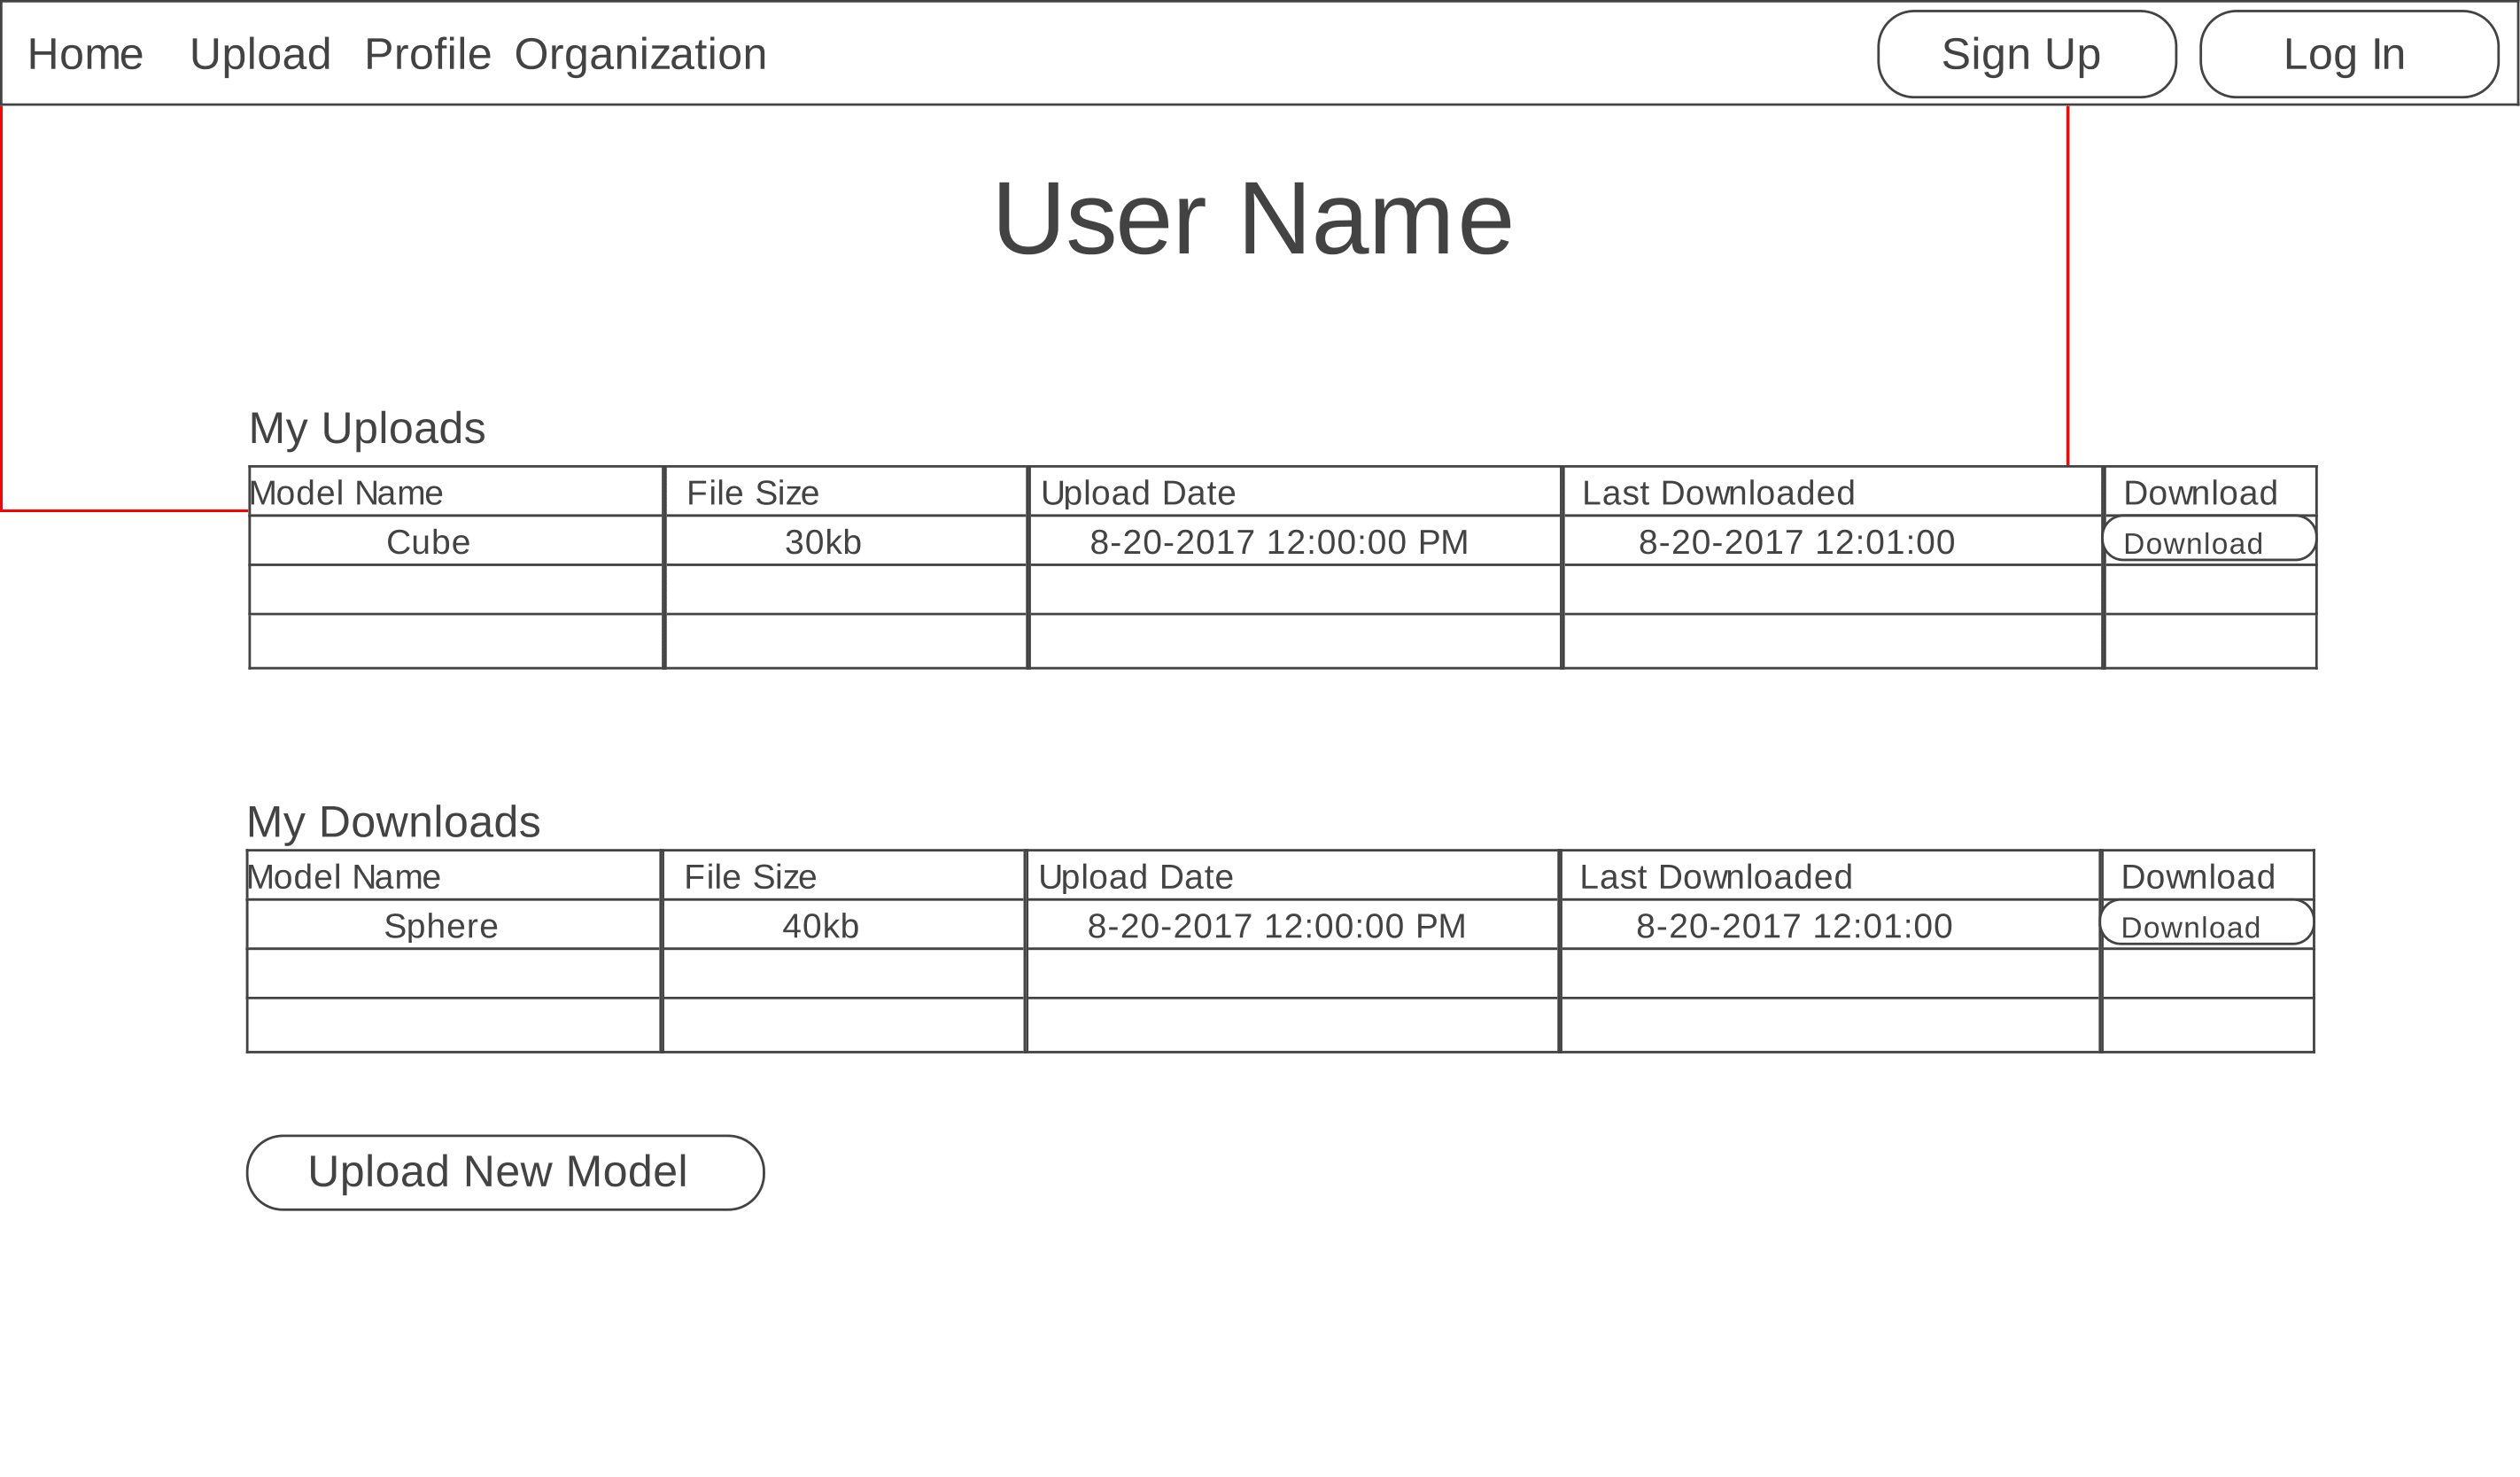
\includegraphics[width=0.6\linewidth]{UserPage}
        \caption{Final design for the My Content page}
    \end{figure}

\subsection{Help Page}
    \hspace{7mm}
    A page displaying simple use instructions for the Augmented Education platform. 
    \ \\
    \label{fig:final_help_page}
    \begin{figure}[H]
        \centering 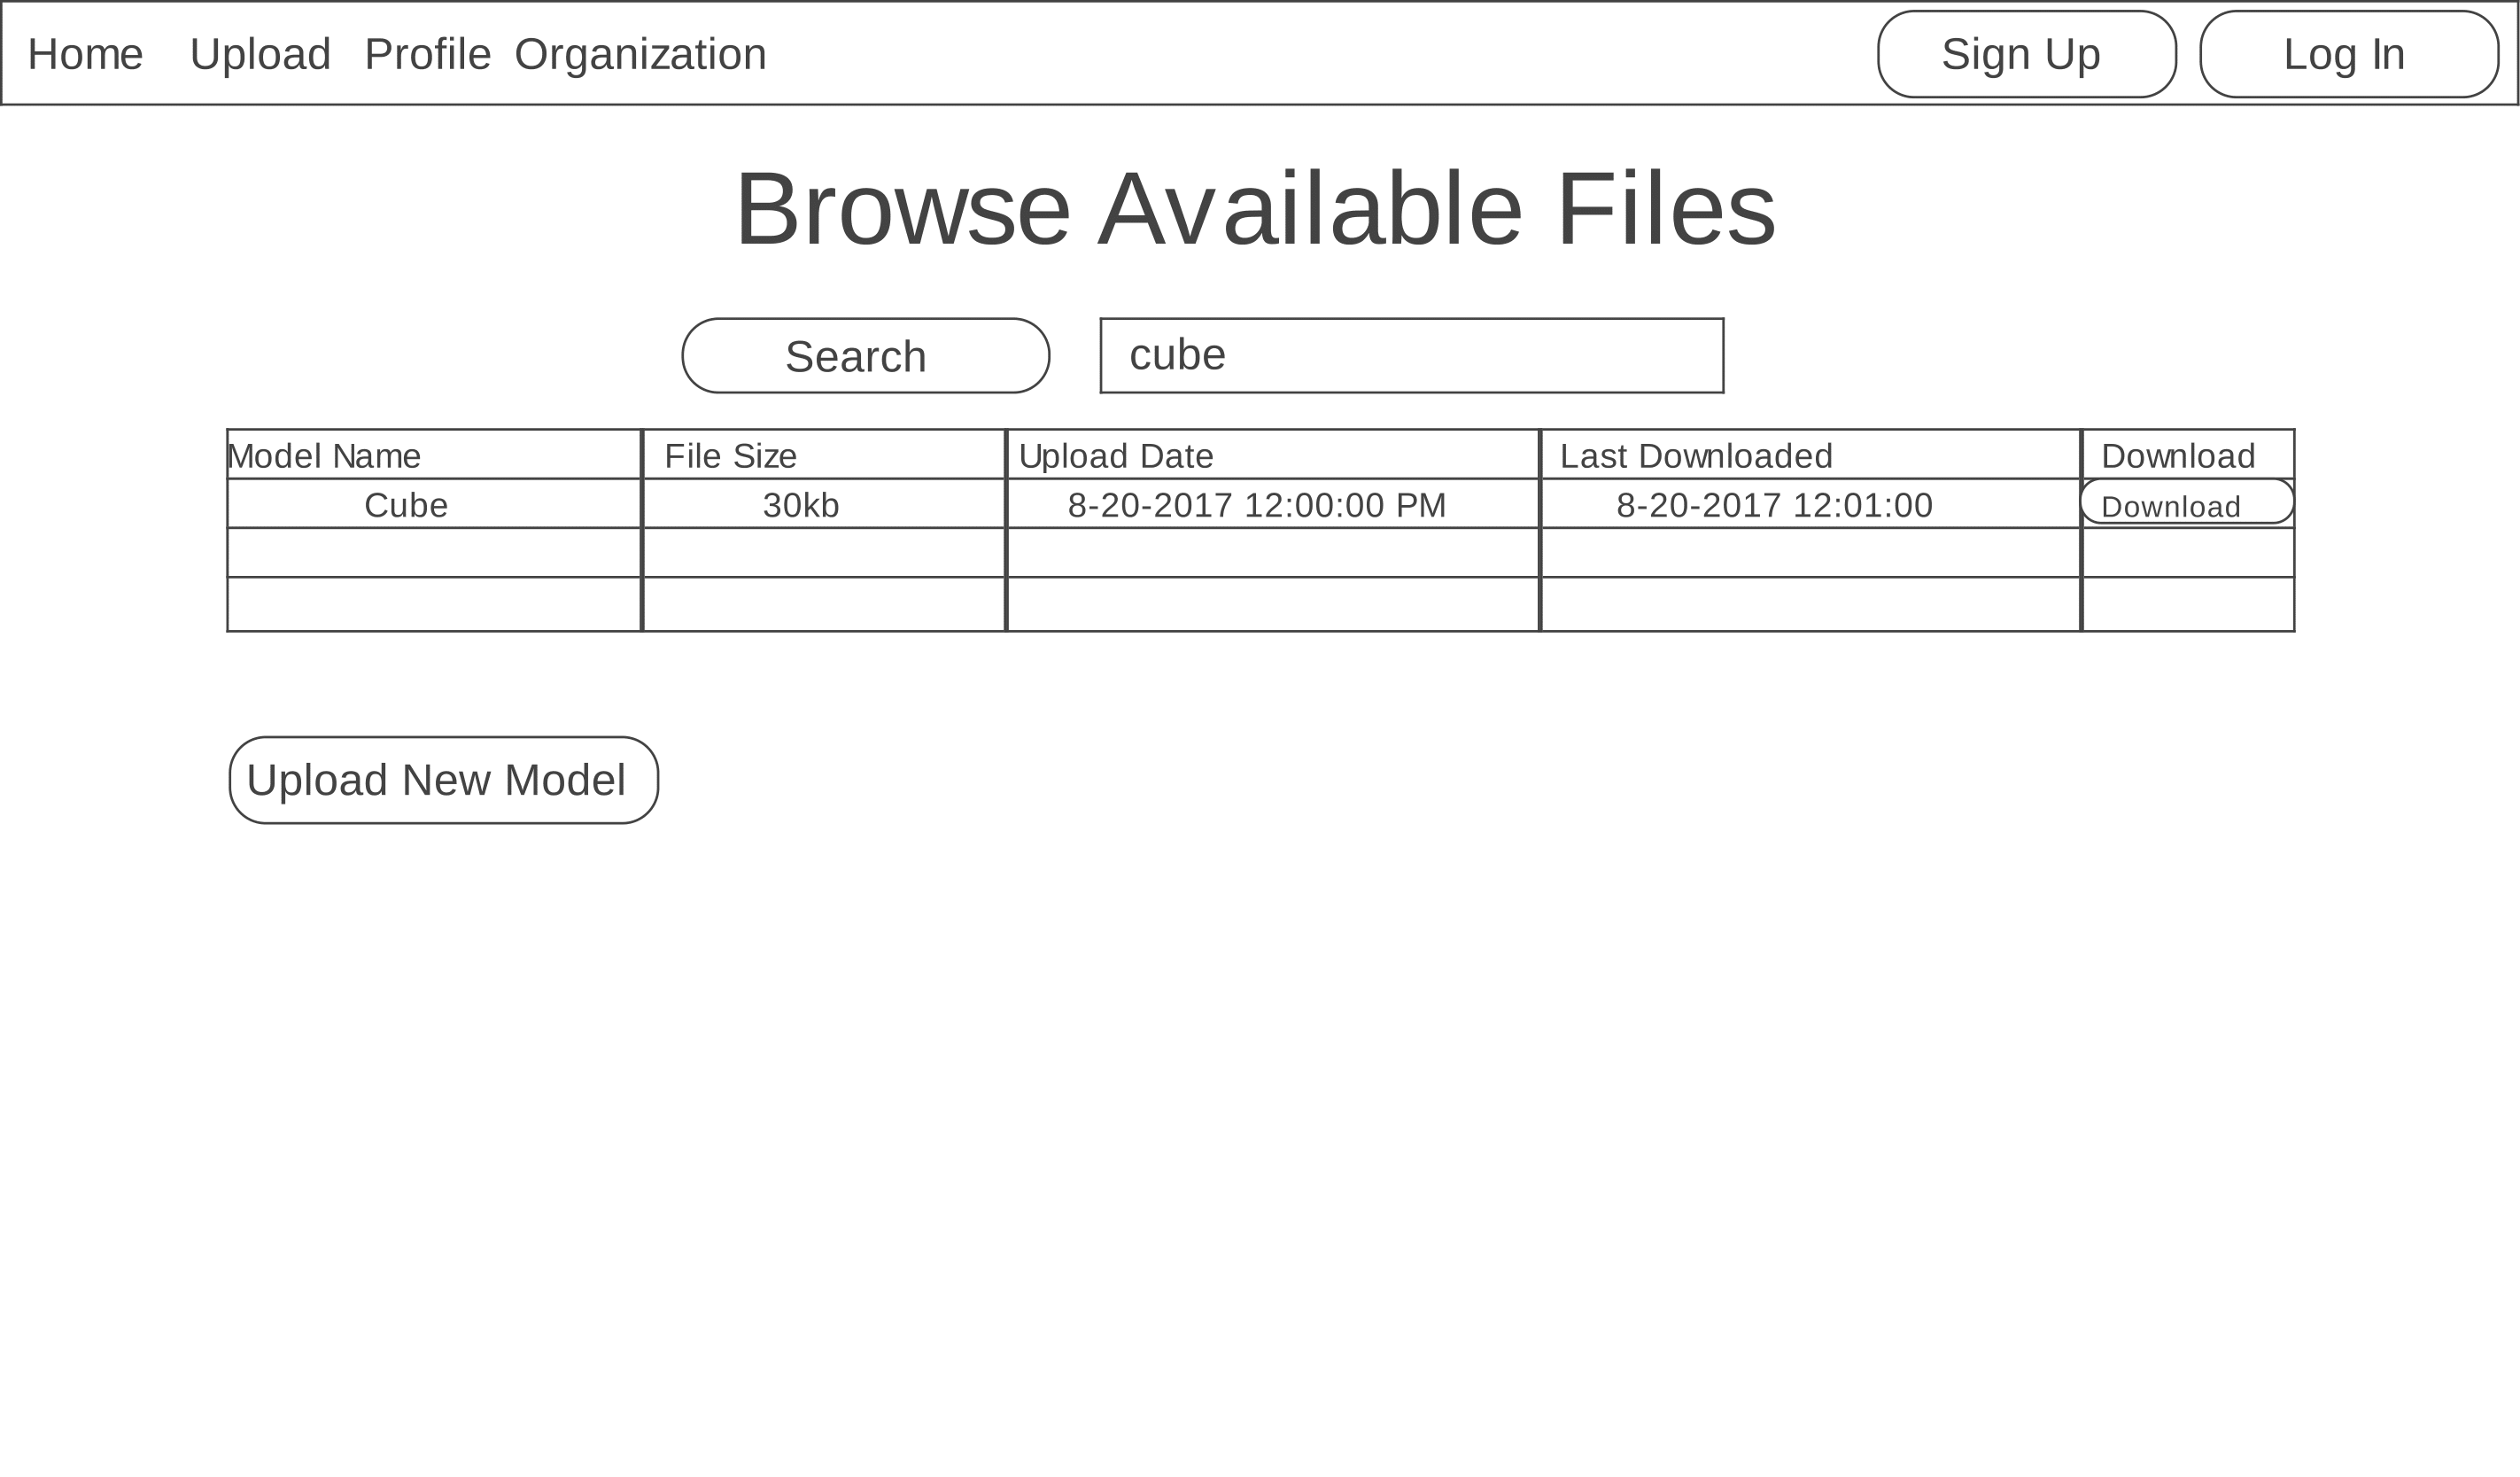
\includegraphics[width=0.6\linewidth]{All}
        \caption{Final design for the Help page}
    \end{figure}

    